\documentclass[12pt,letterpaper]{exam}
\usepackage[lmargin=1in,rmargin=1in,tmargin=1in,bmargin=1in]{geometry}
\usepackage{../style/exams}

% -------------------
% Course & Exam Information
% -------------------
\newcommand{\course}{MAT 107: Exam 3}
\newcommand{\term}{Winter -- 2022}
\newcommand{\examdate}{01/21/2023}
\newcommand{\timelimit}{Time Limit: `$\infty$'}

\setbool{hideans}{false} % Student: True; Instructor: False

% -------------------
% Content
% -------------------
\begin{document}

\examtitle
\instructions{Write your name on the appropriate line on the exam cover sheet. This exam contains \numpages\ pages (including this cover page) and \numquestions\ questions. Check that you have every page of the exam. Answer the questions in the spaces provided on the question sheets. Be sure to answer every part of each question and show all your work. If you run out of room for an answer, continue on the back of the page --- being sure to indicate the problem number.} 
\scores
\bottomline
\newpage

% ---------
% Questions
% ---------
\begin{questions}

% Question 1
\newpage
\question[10] Consider a finite probability space with\dots
	\[
	\begin{aligned}
	P(A)&= 0.35   \qquad& 	&& P(B \text{ and } D)&= 0.15 \\
	P(B)&= 0.40 		& 	&& P(A \text{ and } C)&= 0.10 \\
	P(C)&= 0.65 		& 	&& P(C \text{ and } D)&= 0 \\
	P(D)&= 0.25
	\end{aligned}
	\]

\begin{enumerate}[(a)]
\item Assuming $A$ and $B$ are independent, find $P(A \text{ and } B)$. 
\item Find $P(B \;|\; D)$.
\item Find $P(A \text{ or } C)$.
\item Are $C$ and $D$ independent events? Explain. 
\end{enumerate} \pspace

\sol 
\begin{enumerate}[(a)]
\item Because $A$ and $B$ are independent, we know $P(A \text{ and } B)= P(A) \cdot P(B)$. But then\dots
	\[
	P(A \text{ and } B)= P(A) \cdot P(B)= 0.35 \cdot 0.40= 0.14
	\] \pspace

\item We know that $P(B \text{ and } D)= P(D) P(B \;|\; D)$. But then\dots
	\[
	P(B \;|\; D)= \dfrac{P(B \text{ and } D)}{P(D)}= \dfrac{0.15}{0.25}= 0.60
	\] \pspace

\item 
	\[
	\begin{aligned}
	P(A \text{ or } C)&= P(A) + P(C) - P(A \text{ and } C) \\[0.3cm]
	&= 0.35 + 0.65 - 0.10 \\[0.3cm]
	&= 0.90
	\end{aligned}
	\] \pspace

\item Because the probability space is finite and $P(C \text{ and } D)= 0$, we know that $C$ and $D$ are disjoint events. But disjoint events can never be independent. Therefore, $C$ and $D$ are not independent. 
\end{enumerate}



% Question 2
\newpage
\question[10] Below is a summary of a survey of people about whether or not they preferred to shop in-person or online. \par
	\begin{table}[h]
	\centering
	\begin{tabular}{c|cc||c}
	Age/Shopping & In-Person & Online & Total \\ \hline
	18 -- 30 & 17 & 34 & 51 \\
	30 -- 50 & 54 & 61 & 115 \\
	50$+$ & 40 & 22 & 62 \\ \hline \hline
	Total & 111 & 117 & 228
	\end{tabular}
	\end{table} \par

\begin{enumerate}[(a)]
\item Find the percentage of people surveyed that preferred to shop in-person or were 18--30. 
\item Find the percentage of people surveyed that were 50$+$ and preferred to shop in-person. 
\item Find the percentage of people surveyed that preferred to shop online, if they were 30--50. 
\end{enumerate} \pspace

\sol First, we find the totals of each row and column, which we insert in the table above. 
\begin{enumerate}[(a)]
\item 
	\[
	P(\text{In-Person or 18--30})= \dfrac{111 + 51 - 17}{228}= \dfrac{145}{228} \approx 0.6360
	\] 
Therefore, 63.6\% of people surveyed that preferred to shop in-person or were 18--30. \pspace

\item 
	\[
	P(\text{50+ and In-Person})= \dfrac{40}{228}= \dfrac{10}{57} \approx 0.1754
	\]
Therefore, 17.54\% of people surveyed that were 50$+$ and preferred to shop in-person. \pspace

\item 
	\[
	P(\text{Online} \;|\; \text{30--50})= \dfrac{P(\text{Online and 30--50})}{P(\text{30--50})}= \dfrac{61}{115} \approx 0.5304
	\]
Therefore, 53.04\% of people surveyed that preferred to shop online, if they were 30--50. 
\end{enumerate} 



% Question 3
\newpage
\question[10] Fifty people were surveyed about whether they had read any news online or in print in the last month. Of these people, 27 said they had read news online, 11 said they read news in print, and 5 said they read both. 
	\begin{enumerate}[(a)]
	\item Find the probability that a randomly selected person surveyed read news only online in the last month. 
	\item Find the probability that a randomly selected person surveyed had read no news in the last month. 
	\item Find the probability that a randomly selected person surveyed that read news online in the last month had also read news in print in the last month. 
	\end{enumerate} \pspace

\sol 
\begin{enumerate}[(a)]
\item 
	\[
	P(\text{Only Online})= \dfrac{22}{50}= \dfrac{11}{25} \approx 0.44
	\] \pspace

\item 
	\[
	P(\text{No News})= \dfrac{17}{50} \approx 0.34
	\] \pspace

\item 
	\[
	P(\text{In Print} \;|\; \text{Online})= \dfrac{P(\text{In Print and Online})}{P(\text{Online})}= \dfrac{5}{22 + 5}= \dfrac{5}{27} \approx 0.1852
	\]
\end{enumerate} \vfill

	\[
	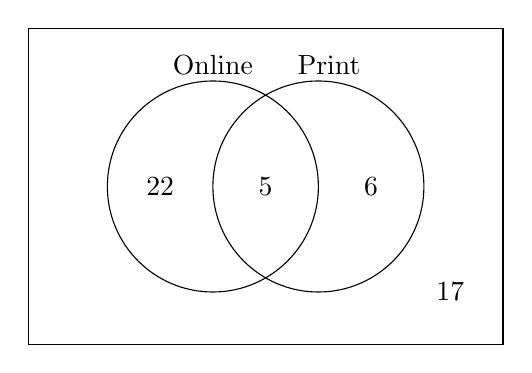
\begin{tikzpicture}[scale=0.67]
	\draw (0,0) rectangle (9,6);
	\draw (3.5,3) circle (2);
	\draw (5.5,3) circle (2);
	
	\node at (3.5,5.3) {Online};
	\node at (5.7,5.3) {Print}; 
	
	\node at (2.5,3) {22};
	\node at (4.5,3) {5};
	\node at (6.5,3) {6};
	\node at (8,1) {17};
	\end{tikzpicture}
	\]



% Question 4
\newpage
\question[10] Suppose in a certain town, 51\% of people are women and 49\% are men. Of men, 56\% tend to lean conservative while only 52\% of women lean conservative. 
	\begin{enumerate}[(a)]
	\item Find the probability that a randomly selected person in the town leans conservative. 
	\item Find the probability that a randomly selected person in the town is a woman or leans conservative. 
	\item Find the probability that a randomly selected person in the town is a man, assuming they do not lean conservative. 
	\end{enumerate} \pspace

\sol 
\begin{enumerate}[(a)]
\item 
	\[
	P(\text{Conservative})= 0.2744 + 0.2652= 0.5396
	\] \pspace

\item 
	\[
	P(\text{Woman or Conservative})= 0.2744 + 0.2652 + 0.2448= 0.7844
	\] \pspace

\item 
	\[
	\begin{aligned}
	P(\text{Man} \;|\; \text{Not Conservative})&= \dfrac{P(\text{Man and Conservative})}{P(\text{Not Conservative})} \\[0.3cm]
	&= \dfrac{0.2744}{0.2156 + 0.2448} \\[0.3cm]
	&= \dfrac{0.2744}{0.4604} \approx 0.5960
	\end{aligned}
	\]
\end{enumerate} \vfill

		\[
		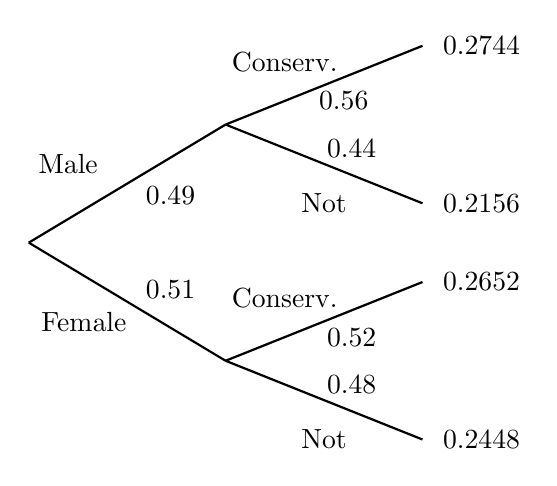
\begin{tikzpicture}[scale= 1.0]
		\def\FirstUpLabel{Male}
		\def\FirstDownLabel{Female}
		\def\SecondUpLabel{Conserv.}
		\def\SecondDownLabel{Not}
		\def\Up{$0.49$}
		\def\Down{$0.51$}
		\def\UpUp{$0.56$}
		\def\UpDown{$0.44$}
		\def\DownUp{$0.52$}
		\def\DownDown{$0.48$}
		\def\first{$0.2744$}
		\def\second{$0.2156$}
		\def\third{$0.2652$}
		\def\fourth{$0.2448$}
		
		\node at (0.5,1) {\FirstUpLabel};	
		\node at (0.7,-1) {\FirstDownLabel};	
		\node at (1.8,0.6) {\Up};
		\node at (1.8,-0.6) {\Down};
		\draw[thick] (0,0) -- (2.5,1.5);
		\draw[thick] (0,0) -- (2.5,-1.5);
		
		\node at (3.25,2.3) {\SecondUpLabel};
		\node at (3.75,0.5) {\SecondDownLabel};
		\node at (4,1.8) {\UpUp};
		\node at (4.1,1.2) {\UpDown};
		\node at (5.75,2.5) {\first};
		\node at (5.75,0.5) {\second};
		\draw[thick] (2.5,1.5) -- (5,2.5);
		\draw[thick] (2.5,1.5) -- (5,0.5);

		\node at (3.25,-0.7) {\SecondUpLabel};
		\node at (3.75,-2.5) {\SecondDownLabel};
		\node at (4.1,-1.2) {\DownUp};
		\node at (4.1,-1.8) {\DownDown};
		\node at (5.75,-0.5) {\third};	
		\node at (5.75,-2.5) {\fourth};	
		\draw[thick] (2.5,-1.5) -- (5,-0.5);
		\draw[thick] (2.5,-1.5) -- (5,-2.5);
		\end{tikzpicture}
		\]



% Question 5
\newpage
\question[10] A certain professor's Wordle scores are given below: \par
	\begin{table}[h]
	\centering
	\begin{tabular}{c||cccccc}
	\# Guesses & 1 & 2 & 3 & 4 & 5 & 6 \\ \hline
	Times Occurred & 0 & 2 & 17 & 48 & 39 & 5 
	\end{tabular}
	\end{table} \par
Find the average number of guesses it takes the professor to guess the word, i.e. the expected number of guesses. \pspace

\sol The professor played a total of $0 + 2 + 17 + 48 + 39 + 5= 111$~games of Wordle. We first find the probability that each guess occurred, which $P(\# \text{ guesses})= \frac{\text{\# times guessed}}{\text{Number Games Played}}$. That gives us the following table: \par
	\begin{table}[h]
	\centering
	\begin{tabular}{c||cccccc}
	\# Guesses & 1 & 2 & 3 & 4 & 5 & 6 \\ \hline
	Times Occurred & 0 & 2 & 17 & 48 & 39 & 5 \\
	Probability & 0 & 0.0180 & 0.1532 & 0.4324 & 0.3514 & 0.0450
	\end{tabular}
	\end{table} \par
Therefore, the average number of guesses, i.e. the expected value, is\dots
	\[
	\begin{aligned}
	EX&= \sum x P(X= x) \\[0.3cm]
	&= 1(0) + 2(0.0180) + 3(0.1532) + 4(0.4324) + 5(0.3514) + 6(0.0450) \\[0.3cm]
	&= 0 + 0.036 + 0.4596 + 1.7296 + 1.757 + 0.27 \\[0.3cm]
	&= 4.2522
	\end{aligned}
	\]



% Question 6
\newpage
\question[10] Consider the following dataset: \par
	\begin{table}[h]
	\centering
	\begin{tabular}{rrrrrrrrrrrrrrrrrrr}
	& $-4$ && $10$ && $1$ && $8$ && $8$ && $21$ && $17$ && $2$ && $0$ \\ 
	$6$ && $14$ && $-3$ && $9$ && $11$ && $20$ && $12$ && $13$ && $-6$ && $16$
	\end{tabular}
	\end{table} \par

\begin{enumerate}[(a)]
\item Find the 5-number summary. 
\item Find the IQR. 
\item Find $P_{32}$. 
\end{enumerate} \pspace

\sol First, we put the data in order:
	\[
	-6 \quad -4 \quad -3 \quad 0 \quad 1 \quad 2 \quad  6 \quad 8 \quad 8 \quad 9 \quad 10 \quad 11 \quad 12 \quad 13 \quad 14 \quad 16 \quad 17 \quad 20 \quad 21
	\]
\begin{enumerate}[(a)]
\item The five-number summary contains the minimum, $Q_1$, median, $Q_3$, and the maximum. The minimum and maximum are clear. Observe there are 19 values. Therefore, the median is the $\frac{19 + 1}{2}= \frac{20}{2}= 10$th value in the dataset, which is 9. To find $Q_1$ and $Q_3$, we find the median of the values below and above the median, respectively. 

There are 9 values above and below the median. Therefore, the median of these sets is the $\frac{9 + 1}{2}= \frac{10}{2}= 5$th value below/above the median, respectively. But then $Q_1= 1$ and $Q_3= 14$. Therefore, the five-number summary is\dots \par
	\begin{table}[!ht]
	\centering
	\begin{tabular}{ccccc}
	Min & $Q_1$ & Median & $Q_3$ & Max \\ \hline
	$-6$ & $1$ & $9$ & $14$ & $21$
	\end{tabular}
	\end{table} \pspace

\item 
	\[
	\text{IQR}= Q_3 - Q_1= 14 - 1= 13
	\] \pspace

\item We know $P_{32}$ is the $19 \cdot \frac{32}{100}= 6.08 \squiggle 7$th value in the dataset. Therefore, $P_{32}= 6$. 
\end{enumerate}



% Question 7
\newpage
\question[10] Consider the following dataset:
	\[
	2 \qquad 4 \qquad 4 \qquad 9
	\]
	
\begin{enumerate}[(a)]
\item Find the mean. 
\item Find the standard deviation. 
\end{enumerate} \pspace

\sol 
\begin{enumerate}[(a)]
\item The mean is\dots
	\[
	\overline{x}= \dfrac{\sum x_i}{n}= \dfrac{2 + 4 + 4 + 9}{4}= \dfrac{19}{4} \approx 4.75
	\] \pspace

\item \phantom{.} \par
	\begin{table}[h]
	\centering
	\begin{tabular}{ccc}
	$x_i$ & $x_i - \overline{x}$ & $(x_i - \overline{x})^2$ \\ \hline
	$2$ & $-2.75$ & $7.5625$ \\
	$4$ & $-0.75$ & $0.5625$ \\
	$4$ & $-0.75$ & $0.5625$ \\
	$9$ & $4.25$ & $18.0625$ \\ \hline
	& Total: & $26.75$
	\end{tabular}
	\end{table} \par
Therefore, the variance is\dots
	\[
	\sigma^2= \dfrac{1}{n - 1} \sum (x_i - \overline{x})^2= \dfrac{1}{4 - 1} \cdot 26.75= \dfrac{1}{3} \cdot 26.75= 8.91667
	\]
But then the standard deviation is $\sigma= \sqrt{\sigma^2}= \sqrt{8.91667} \approx 2.98608$.
\end{enumerate}



% Question 8
\newpage
\question[10] Suppose that the amount of time teenagers spend on their phone per week is normally distributed with mean 752 and standard deviation 279.
	\begin{enumerate}[(a)]
	\item Find the percentage of teens that spend less than 600~minutes on their phone.
	\item Find the percentage of teens that spend more than 600~minutes on their phone. 
	\item How many minutes would a teen minimally need to spend on their phone to be in the greatest 20\% of minutes teenagers spend on their phone per week?
	\end{enumerate} \pspace

\sol 
\begin{enumerate}[(a)]
\item We have\dots
	\[
	z_{600}= \dfrac{600 - 752}{279}= -0.54 \squiggle 0.2946
	\]
Therefore, $P(X < 600)= 0.2946$; that is, 29.46\% of teens spend less than 600~minutes per week on their phone. \pspace

\item We have\dots
	\[
	P(X > 600)= 1 - P(X < 600)= 1 - 0.2946= 0.7054
	\] 
Therefore, 70.54\% of teens spend more than 600~minutes per week on their phone. \pspace

\item If $X$ is the minimum number of minutes needed to be spent on the phone to be in the top 20\% of teenagers. But then $X$ is greater than 80\% of the values in the distribution. But then $z_X \squiggle 0.80$. Examining the $z$-score table, we see that $z_X \approx 0.84$. But then\dots
	\[
	\begin{gathered}
	z_X \approx 0.84 \\[0.3cm]
	\dfrac{X - 752}{279} \approx 0.84 \\[0.3cm]
	X - 752 \approx 234.36 \\[0.3cm]
	X \approx 986.36 \text{ minutes}
	\end{gathered}
	\]
\end{enumerate}



% Question 9
\newpage
\question[10] Suppose that a certain model of car gets an average of 38.6 miles per gallon (mpg) with standard deviation 4.2~mpg. If you took a simple random sample of 45~cars, what is the probability that their average miles per gallon was less than 38~mpg? \pspace

\sol We are given $\mu= 38.6$~miles per gallon and $\sigma= 4.2$~mpg but \textit{not} that the distribution of gas milage is normally distributed. Observe that the sample is a simple random sample and the sample size $n= 45 \geq 30$ is `sufficiently large.' Therefore, the Central Limit Theorem applies. The distribution of sample averages of sample size $n= 45$ is given by\dots
	\[
	N \left( \mu, \, \dfrac{\sigma}{\sqrt{n}} \right)= N \left( 38.6, \, \dfrac{4.2}{\sqrt{45}} \right)= N(38.6, 0.6261)
	\]
But then\dots
	\[
	z_{38}= \dfrac{38 - 38.6}{0.6261}= \dfrac{-0.6}{0.6261} \approx -0.96 \squiggle 0.1685
	\]
But then $P(\overline{X} < 38)= 0.1685$. That is, there is a 16.85\% chance that this sample of 45~cars will get an average gas milage of less than 38~mpg. 



% Question 10
\newpage
\question[10] Suppose that only 3\% of people can identify Moldova on a map. If you randomly surveyed 490~people, what is the probability that more than 8~people surveyed could identify Moldova on a map? \pspace

\sol Each individual can either identify Moldova on the map or not. There are a fixed number of people surveyed, namely $n= 490$. We assume the probability that an individual can identify Moldova is a fixed $p= 0.03$. Finally, we assume that the same was independent. Then the number of individuals surveyed that could identify Moldova on a map, $X$, is given the binomial distribution $B(n, p)= B(490, 0.03)$. We want $P(X > 8)= P(X= 9) + P(X= 10) + \cdots + P(X= 490)$. Of course, this is too many values to compute. Instead, we will use the normal approximation to the binomial distribution. \pspace

Observe that $np= 490(0.03)= 14.7 \geq 10$ and $n(1 - p)= 490(1 - 0.03)= 490(0.97)= 475.3 \geq 10$. Therefore, the normal approximation can be used. We know that $B(n, p) \approx N \big(np, \sqrt{np(1 - p)} \big)$. But then the normal approximation is\dots
	\[
	\begin{aligned}
	N \big(np, \sqrt{np(1 - p)} \big)&= N \big( \, 490(0.03), \, \sqrt{490(0.03)(1 - 0.03)} \, \big) \\[0.3cm]
	&= N(14.7, \sqrt{14.259} \,) \\[0.3cm]
	&= N(14.7, 3.77611)
	\end{aligned}
	\]
Therefore, $B(490, 0.03) \approx N(14.7, 3.77611)$. Now observe\dots
	\[
	z_8= \dfrac{8 - 14.7}{3.77611}= \dfrac{-6.7}{3.77611} \approx -1.77 \squiggle 0.0384
	\]
But then $P(X < 8) \approx 0.0384$. Therefore, $P(X > 8) \approx 1 - P(X < 8) \approx 1 - 0.0384= 0.9616$. Therefore, there is an approximately 96.16\% chance that more than 8 individuals surveyed could identify Moldova on a map. 


\end{questions}
\end{document}